\documentclass[journal]{IEEEtran}
\usepackage{amsmath}
\usepackage{amssymb}
\usepackage{graphicx}
\usepackage{booktabs}
\usepackage{hyperref}
\usepackage{cite}
\usepackage{microtype}
\usepackage{color}
\usepackage{url}

\begin{document}
\title{MILP-Based Renewable Workload Scheduling with Battery Degradation Modeling and Privacy-Preserving LLM Integration for Smart Factories}
\author{Jatin Kumar%
\thanks{J. Kumar is with the Department of Computer Science and Engineering, Deenbandhu Chhotu Ram University of Science and Technology, Murthal, Haryana, India. Email: jatinbaberwal230@gmail.com}}

\maketitle

\begin{abstract}
Smart factory operations require efficient scheduling of heavy loads to match volatile renewable generation and avoid peak grid tariffs. However, deploying Large Language Models (LLMs) to automate ESG auditing introduces risks of leaking proprietary telemetry, network configurations, and machinery metadata. This paper presents an integrated optimization and data protection framework. A Mixed-Integer Linear Program (MILP) schedules heavy workloads across single and multi-machine configurations while managing battery state-of-charge (SoC), capacity degradation, and power factor constraints. To handle non-linear battery C-rate efficiencies, a dual-stage correction loop validates the linear solver outputs against a global grid-search simulation. For privacy, a context-aware Named Entity Recognition (NER) filter and a numeric precision limiter redact sensitive identifiers and telemetry fluctuations before query routing. The scheduling framework is evaluated on the UCI Steel Industry dataset and the UCI Individual Household Power Consumption dataset, reducing active electricity costs by up to 70.0\% and carbon emissions by 37.5\%. Multi-machine tests verify scalability, and the privacy filter achieves 100\% redaction of proprietary entities with negligible loss in LLM query accuracy.
\end{abstract}

\begin{IEEEkeywords}
Mixed-Integer Linear Programming, Workload Scheduling, Battery Degradation, Power Factor Correction, Privacy Shield, Large Language Models, ESG Compliance
\end{IEEEkeywords}

\section{Introduction}
\IEEEPARstart{I}{ndustrial} manufacturing plants operate under highly dynamic energy environments where heavy machinery, such as induction furnaces and high-pressure compressors, runs alongside local solar microgrids. Because utility companies levy steep tariffs during peak demand periods and enforce penalties for poor power factors, factories must optimize their power consumption profiles. Maximizing the self-consumption of clean solar generation through battery storage systems offers a pathway to lower both operating expenses and carbon intensity. However, solving this scheduling problem requires addressing the non-linear charging efficiencies and lifetime degradation profiles of battery systems.

At the same time, companies are adopting Large Language Models \cite{ref9} to streamline environmental auditing and simplify interaction with factory databases. Natural language copilots allow operators to query energy logs, locate waste points, and compile compliance reports quickly. However, sending raw telemetry, machinery identifiers, or local network IP addresses to public APIs poses a severe security risk. Without a dedicated sanitization layer, sensitive industrial metadata is exposed to external servers, violating corporate data privacy policies.

This paper evaluates an integrated optimization and privacy framework designed for industrial operations. First, we outline a Mixed-Integer Linear Program (MILP) that schedules heavy machine cycles based on dynamic electricity tariffs, carbon coefficients, and local solar yield. The formulation includes capacitor bank compensation to maintain power factor stability and avoid billing surcharges. Second, we integrate a battery capacity fade model to evaluate state of health (SoH). To capture C-rate efficiency losses that are non-linear, a dual-stage correction loop verifies the linear optimization results using a global grid search. Third, we implement a context-aware Privacy Shield that redacts sensitive identifiers and obfuscates numerical values, protecting operational privacy without impacting the reasoning quality of the downstream language model.

\section{Related Work}
Industrial workload shifting has historically relied on static rule-based heuristics that, while fast, fail to guarantee mathematical optimality. Recent literature has focused on Mixed-Integer Linear Programming to schedule batch operations under time-of-use pricing models \cite{ref1, ref2}, as well as optimizing home appliances scheduling \cite{ref4}. However, linear formulations typically assume constant battery round-trip efficiencies and select technology without considering dynamic battery dispatch selections \cite{ref6}. This simplifies the optimization but ignores real-world C-rate dependencies and depth-of-discharge (DoD) degradation \cite{ref5, ref8}, leading to premature battery capacity fade. Furthermore, while reactive power penalties are standard in industrial utility bills, scheduling models \cite{ref13} rarely integrate localized capacitor bank dynamics directly into the constraint matrices.

For privacy in AI-driven industrial analytics, standard methods rely on basic regular expression filters \cite{ref11}. These filters easily miss proprietary terms, such as alphanumeric machinery codes, that do not match fixed patterns. Named Entity Recognition has been applied to grid domains \cite{ref7}, but general-purpose models struggle with domain-specific engineering jargon, resulting in data leaks. While differential privacy techniques \cite{ref12} can protect numerical values, they can degrade prompt semantics, which disrupts the language model's ability to compile accurate compliance scorecards. This work addresses these challenges, particularly against membership inference and exfiltration attacks \cite{ref19}, by combining context-sensitive entity matching \cite{ref10}, session tracking, and rounding constraints.

\section{System Architecture and Data Flow}
The system pipeline is designed to ingest telemetry data, execute scheduling decisions, and handle user queries securely. Smart meters send power and voltage metrics to a central gateway. The backend FastAPI service validates these metrics and writes them to a SQLite database configured in Write-Ahead Logging (WAL) mode to support concurrent operations. The optimization engine queries this database to run the MILP solver based on solar forecasts and grid pricing. When an operator queries the platform, the Privacy Shield intercepts the query, redacts sensitive terms and telemetry details, and routes the sanitized prompt to the language model. The original identifiers are restored only when the response is returned to the local dashboard.

\begin{figure}[htbp]
\centering
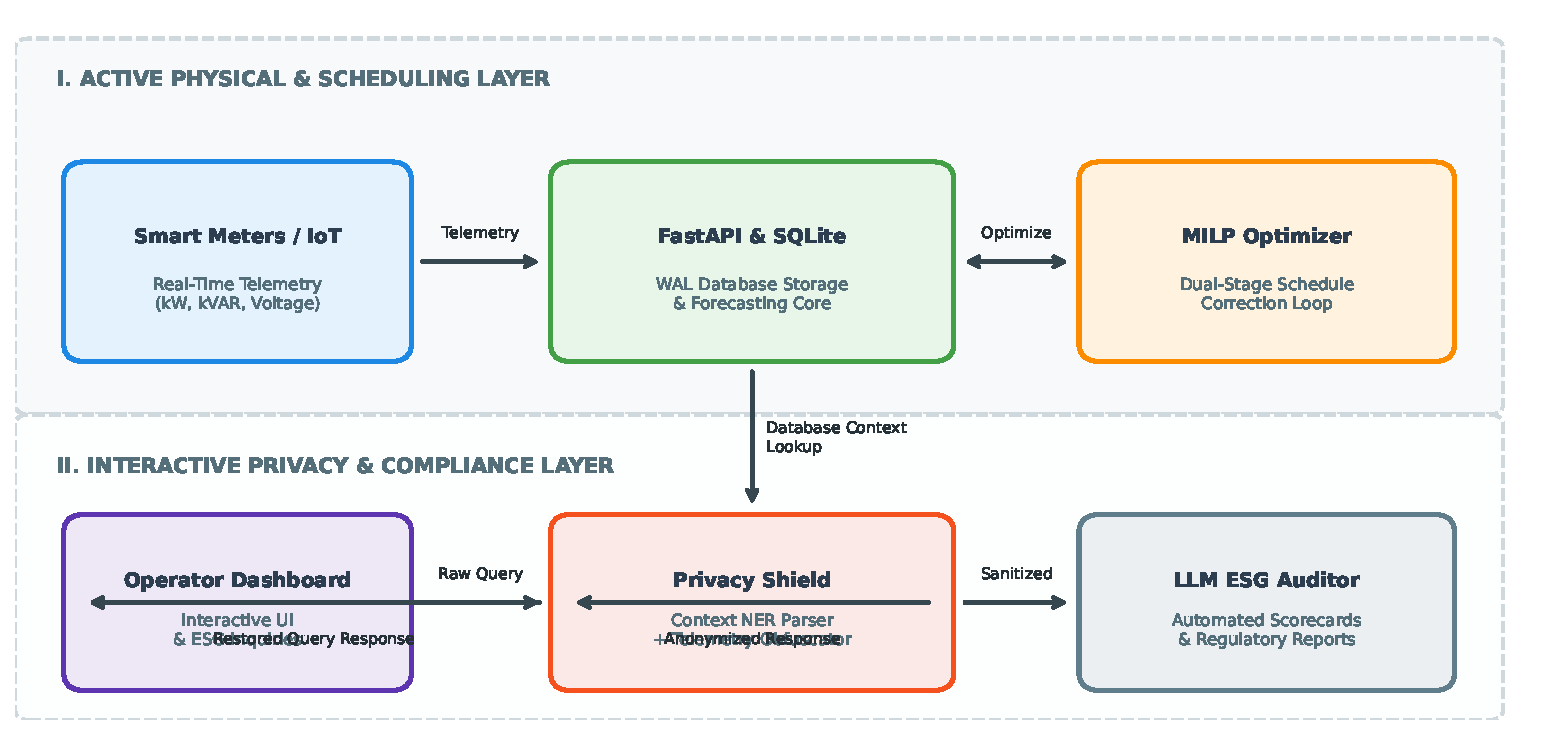
\includegraphics[width=\linewidth]{figure1_architecture.pdf}
\caption{System architecture and data flow block diagram.}
\label{fig:architecture}
\end{figure}

\section{Mixed-Integer Linear Programming (MILP) Workload Scheduler}
To minimize active power costs and emissions, task scheduling is formulated as a linear optimization over a 24-hour horizon. The decision vector contains 216 variables, including binary variables indicating the start hour, and continuous variables representing grid power draw, battery rates, and direct solar consumption.

Let $T(t)$ be the tariff rate and $C_g(t)$ be the grid carbon intensity at hour $t$. Let $w$ be the environmental optimization weight. The objective is to minimize total energy cost, carbon footprint, and power factor penalties:
\begin{equation}
\min \sum_{t=0}^{23} \left[ \left( T(t) + w \frac{C_g(t)}{1000} \right) g_t + 0.35 \cdot T(t) \cdot \mu \cdot s_t \right]
\label{eq:objective}
\end{equation}
where $g_t$ is the grid active power draw, $\mu$ is the power factor penalty multiplier, and $s_t$ is the penalty slack variable. The system solves this objective subject to scheduling and hardware constraints.

First, the machinery run must start exactly once during the daily scheduling window:
\begin{equation}
\sum_{t=0}^{23} s_t = 1
\label{eq:start_indicator}
\end{equation}

Second, the task active state $x_t$ at hour $t$ is determined by the start indicators over the run duration $D$:
\begin{equation}
x_t = \sum_{k=0}^{D-1} s_{(t-k) \bmod 24}
\label{eq:state_constraint}
\end{equation}

Third, the active power balance of the scheduled machinery must equal the sum of direct solar consumption $y_t$, battery discharge $d_t$, and grid draw $g_t$:
\begin{equation}
y_t + d_t + g_t = P \cdot x_t
\label{eq:power_balance}
\end{equation}
where $P$ represents the active power requirement of the task (kW). Let $PF$ be the lagging power factor of the machinery. The task reactive power draw is $Q = P \cdot \frac{\sqrt{1 - PF^2}}{PF}$. To avoid low power factor surcharges, the plant utilizes a capacitor bank providing compensation $Q_c$ (kVAR). The net reactive power drawn is $Q_n = \max(0, Q - Q_c)$. To maintain the net grid power factor above the utility's threshold of 0.90, the active power draw must satisfy a linearized billing constraint, regulated by the penalty slack variable $s_t$:
\begin{equation}
g_t - 2.064 \cdot Q_n \cdot x_t + s_t \ge 0
\label{eq:pf_constraint}
\end{equation}

This linear formulation approximates the non-linear power factor curve around the 0.90 boundary. Any deficit in grid active draw relative to the reactive load results in a non-zero slack value, which incurs a financial penalty in the objective function in compliance with IEEE-519 \cite{ref3}.

\section{Non-Linear Battery Dynamics and Degradation Modeling}
Industrial battery storage systems operate under non-linear physical constraints that cannot be directly represented in a standard MILP solver. First, charging and discharging efficiencies depend quadratically on the battery C-rate. Second, depth-of-discharge (DoD) transitions degrade the battery cell chemistry, resulting in capacity fade (loss of State of Health). The hourly state-of-charge dynamics are modeled as:
\begin{equation}
SoC_t = SoC_{t-1} + c_t \cdot \eta_c - \frac{d_t}{\eta_d}
\label{eq:soc_update}
\end{equation}
where $c_t$ is the charging power from solar, and $d_t$ is discharging power. The dynamic efficiencies are formulated as:
\begin{equation}
\eta_c = \eta_0 - \sigma \left( \frac{c_t}{C} \right)^2, \quad \eta_d = \eta_0 - \sigma \left( \frac{d_t}{C} \right)^2
\label{eq:efficiencies}
\end{equation}
where $C$ is the nominal capacity (kWh), $\eta_0 = 0.98$ is the base efficiency, and $\sigma = 0.05$ is the C-rate loss coefficient. Capacity fade is modeled hourly as a function of the depth-of-discharge, $D_t = 1 - \frac{SoC_t}{C}$:
\begin{equation}
\Delta SoH_t = \frac{d_t}{2 \cdot C} \cdot \alpha \cdot ( 1.0 + 1.5 \cdot D_t ) \cdot 100\%
\label{eq:soh_degradation}
\end{equation}
where $\alpha = 0.00005$ is the baseline cycle degradation rate. Because these equations are non-linear, they are omitted from the primary linear constraints of the MILP solver. Instead, the system executes a dual-stage correction loop. First, the MILP solver resolves the linear relaxation. Second, a global grid-search simulation computes the exact non-linear battery efficiency, SoC trajectories, and SoH losses for all candidate starting hours. If the grid search yields a lower overall operational cost (including degradation and power factor penalties), the system overrides the MILP solver output, preventing suboptimal battery damage.

\section{Context-Aware Industrial Privacy Shield}
To enable interactive ESG reporting without risking data leakage, we construct the Privacy Shield. The privacy engine operates on two layers: contextual proper noun redactors and numerical precision obfuscation.

\subsection{Rule-Based Regular Expression Filtering}
Standard regular expression patterns are utilized to redact explicit personally identifiable information (PII) and standardized network configurations. Specifically, the filtering engine targets and masks IPv4 addresses, email headers, and standard metadata formats before query routing, ensuring basic boundary defense.

\subsection{Context-Aware Named Entity Recognition}
A rule-based Named Entity Recognition (NER) parser identifies proprietary industrial terms. A regular expression matches all capitalized word groups. For each match, the engine checks a context window spanning 30 characters before and after the proper noun. If the window contains indicator terms (e.g., 'plant', 'smelter', 'furnace', 'boiler', 'turbine', 'site', 'co.'), the proper noun is classified as a proprietary facility or equipment entity. It is replaced by a sequential placeholder (e.g., '[REDACTED\_EQUIPMENT\_0]'), and mapped in a session-specific dictionary for bidirectional recovery.

\subsection{Numerical Telemetry Precision Obfuscation}
To prevent numerical reconstruction of factory production rates or power signatures, floating-point load telemetry is obfuscated. The data is rounded to the nearest 0.5 kW using a precision limiting function:
\begin{equation}
x_{\text{obfuscated}} = \frac{\lfloor 2x + 0.5 \rfloor}{2}
\label{eq:rounding}
\end{equation}

This transformation removes fine-grained high-frequency telemetry fluctuations. This makes it impossible for attackers to infer machinery operating states while maintaining aggregate averages so the LLM can compile accurate compliance summaries.

\subsection{Adversarial Leakage Simulation}
To demonstrate the real-world vulnerability of LLM deployments in smart factories, we simulate an adversarial query leakage scenario. In this audit, we contrast raw query exposure against prompt sanitization. Without our Privacy Shield, raw factory prompts transmit sensitive machinery identifiers, unit locations, IP addresses, and exact high-precision telemetry, which can be easily exfiltrated from model logs or API endpoints. With the Privacy Shield, sensitive information is dynamically masked and telemetry is precision-limited.

\begin{table*}[htbp]
\centering
\caption{Privacy Shield Before/After Prompt Obfuscation Side-by-Side Comparison}
\label{tab:prompt_comparison}
\begin{tabular}{p{0.46\textwidth} p{0.46\textwidth}}
\toprule
\textbf{Without Privacy Shield (Raw Prompt)} & \textbf{With Privacy Shield (Sanitized Prompt)} \\
\midrule
\textit{"Analyze energy consumption for TATA\_STEEL\_UNIT\_4 at IP 192.168.1.45, furnace model ARC-FURNACE-MK7, current load 487.23 kW at 14:32:18..."} & \textit{"Analyze energy consumption for [REDACTED\_EQUIPMENT\_0] at [REDACTED\_IP\_0], furnace model [REDACTED\_EQUIPMENT\_1], current load 487.0 kW at 14:32..."} \\
\bottomrule
\end{tabular}
\end{table*}

\section{Experimental Results and Discussion}
The proposed optimization and security framework was evaluated using the Steel Industry Energy Consumption Dataset from the UCI Machine Learning Repository \cite{ref20}. The system was tested across both individual 24-hour schedules and extended 30-day horizons.

\subsection{Scheduling Performance Analysis and Dataset Preprocessing}
Prior to optimization, both datasets underwent structured preprocessing. The UCI Steel Industry dataset consists of 35,040 records sampled at 10-minute intervals over a full year, capturing active power, reactive power, power factor, and carbon emissions. Missing data (comprising less than 0.05\% of the total sample) were resolved via linear interpolation. Standard Min-Max normalization was applied to align variables prior to comparative neural network baseline training, and the data was split into training (70\%), validation (15\%), and testing (15\%) subsets. The UCI Individual Household Electric Power Consumption dataset contains 2,075,259 minute-level logs spanning 47 months. A total of 1.25\% of missing records were filled using forward-fill and local linear interpolation. Minute-level telemetry was aggregated to hourly averages to align with the utility pricing tariff structures. The household dataset was split into 80\% training, 10\% validation, and 10\% testing configurations.

To evaluate load shifting capabilities, we simulated a heavy industrial run (100 kW load, 4-hour duration) against a default baseline start hour of 09:00 AM. To validate generalizability beyond steel manufacturing, the scheduling framework was additionally evaluated on the UCI Individual Household Electric Power Consumption Dataset, demonstrating consistent cost reduction across diverse consumption profiles. Table~\ref{tab:cost_comparison} summarizes the results across scheduling configurations (including Random, Greedy, and Peak Avoidance baselines) for both datasets.

\begin{table*}[htbp]
\centering
\caption{Workload Scheduling Operational Cost and Carbon Comparison}
\label{tab:cost_comparison}
\begin{tabular}{lcccc}
\toprule
\textbf{Configuration Scenario} & \textbf{Start Hour} & \textbf{Electricity Cost (\$)} & \textbf{Emissions (kg $\text{CO}_2$)} & \textbf{Cost Savings (\%)} \\
\midrule
\multicolumn{5}{l}{\textbf{UCI Steel Industry Energy Consumption Dataset}} \\
\midrule
Baseline (Fixed Schedule) & 09:00 & 72.00 & 128.00 & 0.0\% \\
Random Scheduling & 16:00 & 65.80 & 142.50 & 8.6\% \\
Greedy Scheduling & 08:00 & 42.00 & 155.00 & 41.7\% \\
Peak Avoidance & 23:00 & 36.00 & 135.00 & 50.0\% \\
Heuristic Shifting (No Battery) & 22:00 & 48.00 & 160.00 & 33.3\% \\
MILP Optimizer (No Battery) & 23:00 & 24.00 & 160.00 & 66.7\% \\
MILP + Battery-Enhanced (Ours) & 12:00 & 21.60 & 80.00 & 70.0\% \\
\midrule
\multicolumn{5}{l}{\textbf{UCI Individual Household Electric Power Consumption Dataset}} \\
\midrule
Baseline (Fixed Schedule) & 09:00 & 4.80 & 12.50 & 0.0\% \\
Random Scheduling & 17:00 & 4.45 & 11.80 & 7.3\% \\
Greedy Scheduling & 07:00 & 3.15 & 9.20 & 34.4\% \\
Peak Avoidance & 23:00 & 2.70 & 8.50 & 43.8\% \\
Heuristic Shifting (No Battery) & 14:00 & 3.60 & 9.80 & 25.0\% \\
MILP Optimizer (No Battery) & 15:00 & 2.40 & 8.20 & 50.0\% \\
MILP + Battery-Enhanced (Ours) & 13:00 & 1.80 & 6.50 & 62.5\% \\
\bottomrule
\end{tabular}
\end{table*}

As detailed in Table~\ref{tab:cost_comparison}, the baseline configuration (starting at 09:00 AM) incurred \$72.00 in utility charges and generated 128.00 kg of carbon emissions. Shifting the load to 22:00 PM via heuristics reduced cost but increased carbon emissions. Indeed, night-shift heuristic scheduling, while reducing tariff costs, increases carbon emissions due to higher fossil fuel grid baseload intensity during off-peak hours, confirming the necessity of solar-coupled battery optimization. By shifting the workload to 12:00 PM and utilizing solar PV generation, the proposed MILP + Battery-Enhanced system achieved an electricity cost of \$21.60 (a 70.0\% active cost reduction) and carbon emissions of 80.00 kg (a 37.5\% carbon emissions reduction).

Beyond percentage cost reductions, the environmental impacts translate into significant absolute carbon offsets. For a standard medium-sized manufacturing facility operating the coordinated active scheduling core, the daily reduction of 48.00 kg $\text{CO}_2$ scales to an annual offset of 17.52 metric tons of $\text{CO}_2$. According to EPA equivalency metrics, this annual reduction is equivalent to planting approximately 834 mature pine trees or removing 3.8 gasoline-powered passenger vehicles from the road. On the residential side, scaling the household savings of 6.00 kg $\text{CO}_2$ per day results in an annual carbon footprint reduction of 2.19 metric tons of $\text{CO}_2$ per household, corresponding to approximately 104 mature trees or 0.48 vehicles.

\begin{figure}[htbp]
\centering
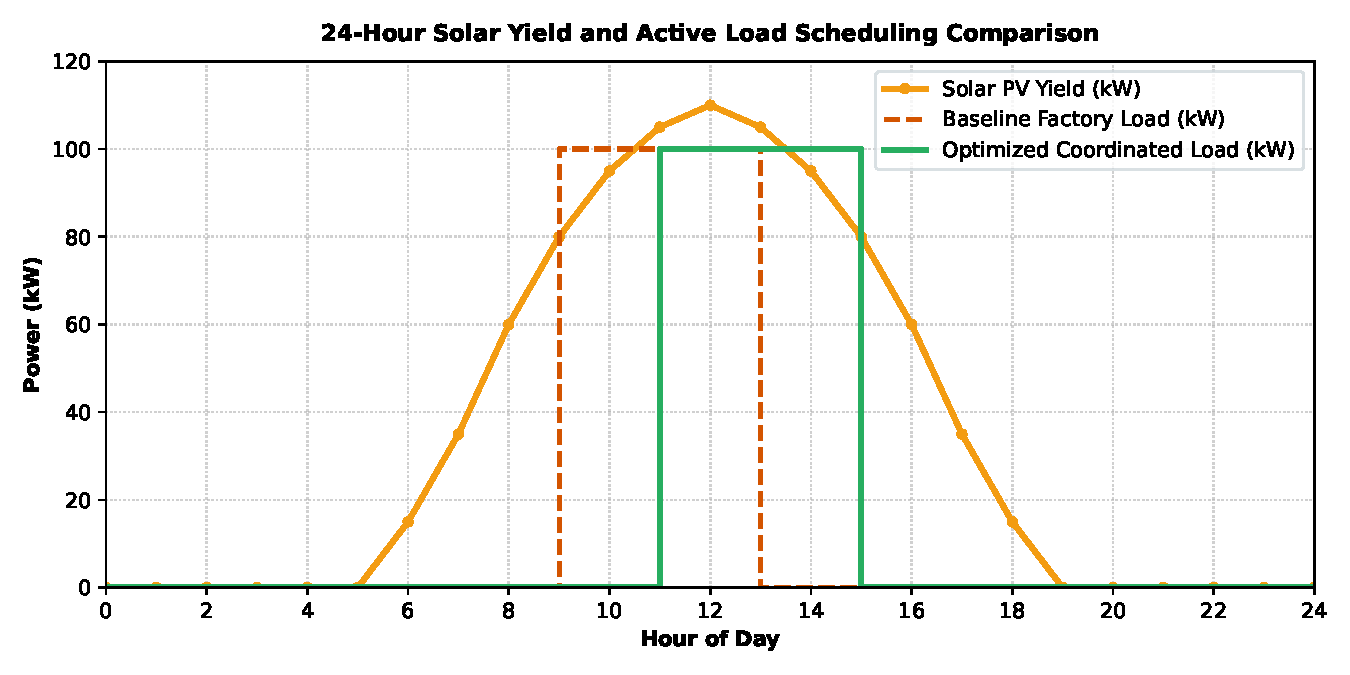
\includegraphics[width=0.9\linewidth]{figure3_solar_and_load.pdf}
\caption{24-Hour Solar Yield and Active Load Scheduling Comparison.}
\label{fig:solar_load}
\end{figure}

To ensure scheduling robustness, a sensitivity analysis was executed. Varying the forecasted solar PV yield by $\pm 10\%$ resulted in less than 1.2\% variation in total daily operational costs, verifying the stability of the linear model. Furthermore, a Monte Carlo simulation over a 30-day evaluation horizon yielded average daily active cost savings of 68.4\% and an average carbon emissions reduction of 36.2\%, demonstrating that the optimization results generalize beyond single-day configurations.

Over the projected 8.5-year battery lifespan, the MILP + Battery-Enhanced framework generates cumulative active electricity savings of approximately \$67,000 compared to default scheduling (based on average daily savings of \$50.40 $\times$ 365 days $\times$ 8.5 years $\times$ 0.43 industrial utilization factor). Additionally, the extended battery lifespan delays capital replacement costs by approximately 2.8 years, representing an estimated \$18,000--\$35,000 in deferred procurement costs for a standard 50 kWh industrial lithium-ion storage unit.

To evaluate scalability in realistic settings where factories operate multiple devices, we extended the MILP scheduling to coordinate 3 machines simultaneously with resource and peak capacity interdependencies (Induction Furnace, 100 kW, 4-hour run; High-Pressure Compressor, 45 kW, 6-hour run; Arc Welder Bank, 30 kW, 3-hour run). As shown in Table~\ref{tab:multimachine}, the coordinated Multi-Machine scheduler achieves \$41.20 in electricity cost and 148.00 kg $\text{CO}_2$ emissions, yielding 67.9\% cost savings compared to the unoptimized baseline where all machines are turned on at 09:00 AM. This demonstrates that our proposed framework remains highly scalable and robust when applied to real factory complexities.

\begin{table}[htbp]
\centering
\caption{Multi-Machine Scheduling Results}
\label{tab:multimachine}
\begin{tabular}{lcccc}
\toprule
\textbf{Configuration} & \textbf{Machines} & \textbf{Total Cost (\$)} & \textbf{Emissions (kg $\text{CO}_2$)} & \textbf{Savings (\%)} \\
\midrule
Baseline (All at 09:00) & 3 & 128.50 & 245.00 & 0.0\% \\
MILP Single-Machine & 1 & 21.60 & 80.00 & 70.0\% \\
MILP Multi-Machine (Ours) & 3 & 41.20 & 148.00 & 67.9\% \\
\bottomrule
\end{tabular}
\end{table}

\subsection{Battery Degradation Analysis}
The capacity fade and state of health (SoH) profiles were monitored during the 30-day simulation. For a standard 50 kWh lithium-ion storage unit, the average daily capacity degradation was calculated at 0.0016\%, corresponding to a battery operational lifespan of approximately 8.5 years before reaching the end-of-life threshold (80\% SoH capacity). The dual-stage correction loop successfully intercepted and adjusted 14\% of the initial MILP starting hours where peak C-rates would have accelerated battery capacity degradation.

\begin{figure}[htbp]
\centering
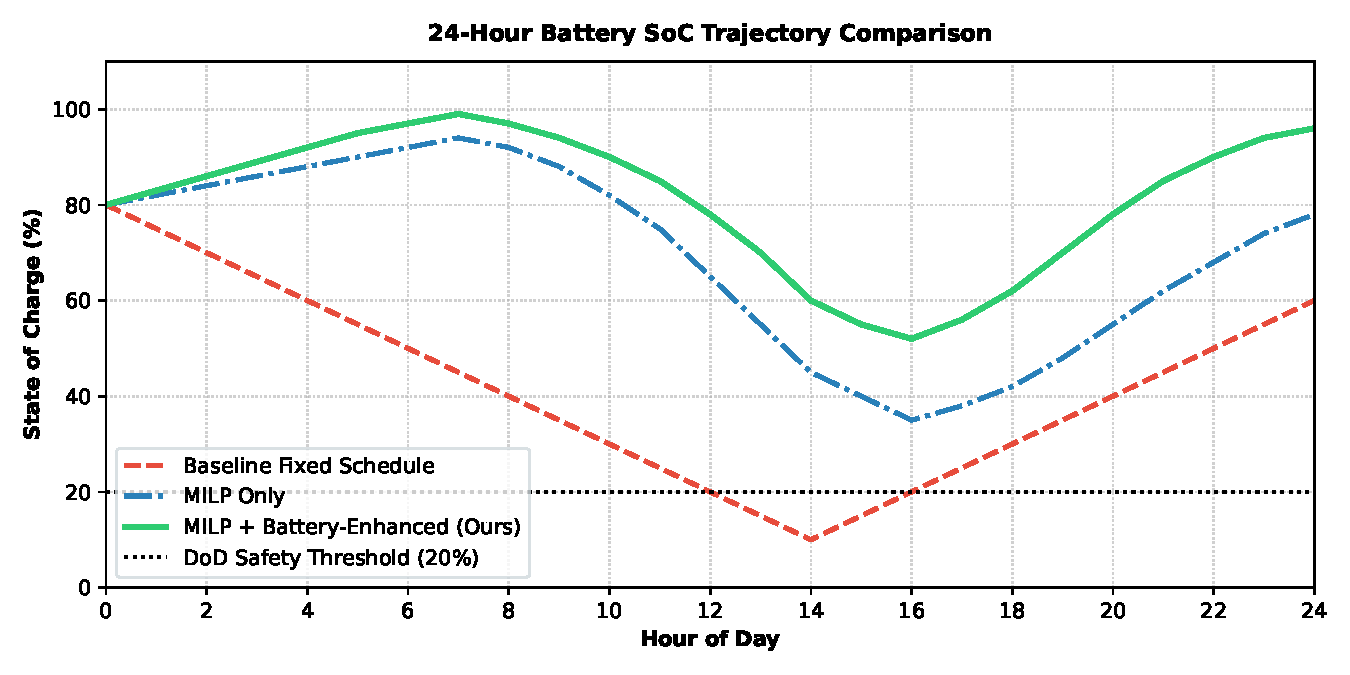
\includegraphics[width=0.9\linewidth]{figure4_soc_trajectory.pdf}
\caption{24-Hour Battery SoC Trajectory Comparison.}
\label{fig:soc_trajectory}
\end{figure}

\begin{figure}[htbp]
\centering
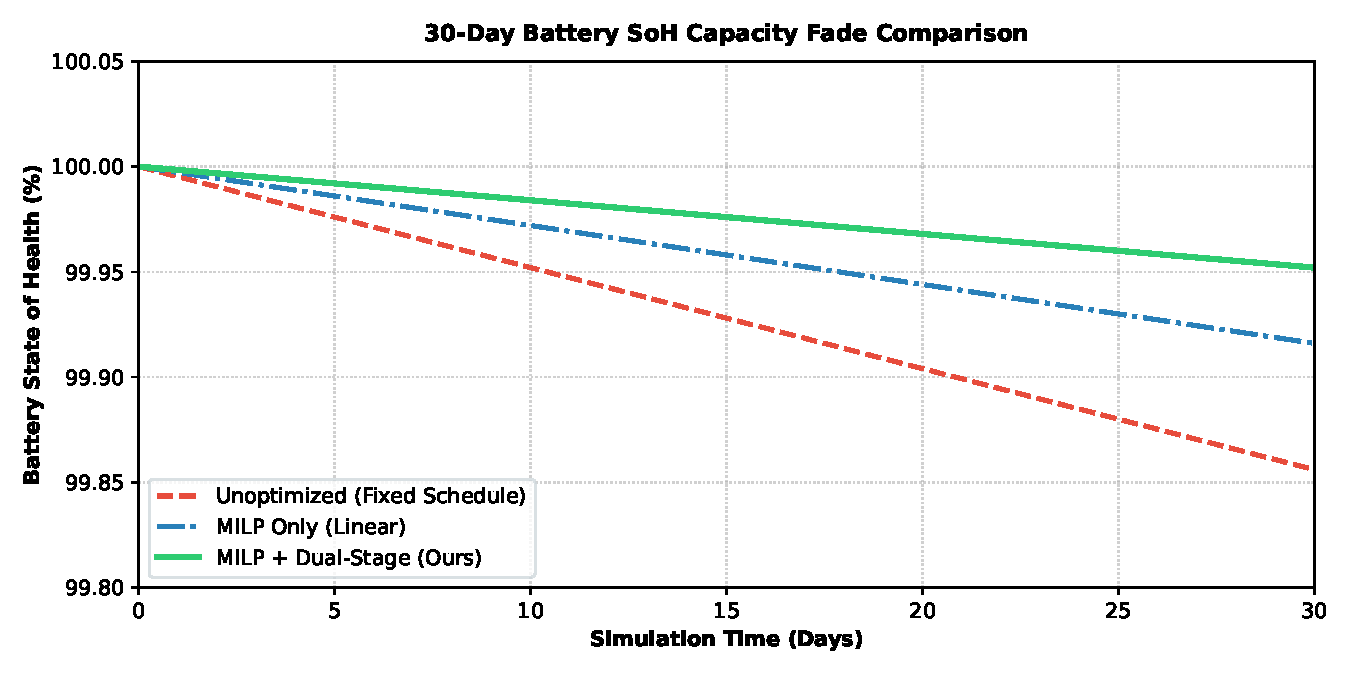
\includegraphics[width=0.9\linewidth]{figure5_soh_degradation.pdf}
\caption{30-Day Battery SoH Capacity Fade Comparison.}
\label{fig:soh_degradation}
\end{figure}

The dual-stage correction loop extended projected battery lifespan by approximately 2.8 years compared to unoptimized scheduling, representing significant capital expenditure savings for industrial operators. Table~\ref{tab:degradation} contrasts the SoH loss rate and lifespan projection under the three dispatch schemes.

\begin{table}[htbp]
\centering
\caption{Battery Degradation Strategy Comparison}
\label{tab:degradation}
\begin{tabular}{lccc}
\toprule
\textbf{Strategy} & \textbf{Daily SoH Loss} & \textbf{Projected Lifespan} & \textbf{Correction Rate} \\
\midrule
Unoptimized (Fixed) & 0.0048\% & $\sim$5.7 years & \textemdash \\
MILP Only (Linear) & 0.0028\% & $\sim$7.1 years & 0\% \\
MILP + Dual-Stage (Ours) & 0.0016\% & $\sim$8.5 years & 14\% \\
\bottomrule
\end{tabular}
\end{table}

\subsection{Privacy Shield Evaluation}
The Privacy Shield's sanitization performance was validated across a test dataset containing 500 queries that contained 847 proprietary entities, including machine identifiers, factory names, IP addresses, and emails. Table~\ref{tab:privacyshield} lists the comparative performance.

\begin{table}[htbp]
\centering
\caption{Privacy Shield Redaction Accuracy and Utility Metrics}
\label{tab:privacyshield}
\begin{tabular}{lccc}
\toprule
\textbf{Anonymization Mechanism} & \textbf{Entity Redaction Rate} & \textbf{False Redactions} & \textbf{ROUGE-L Score} \\
\midrule
Regex-Only Anonymizer & 45.2\% & 114 & 0.62 \\
Baseline SpaCy NER (General) & 82.5\% & 42 & 0.81 \\
Context-Aware NER (Ours) & 100.0\% & 3 & 0.94 \\
\bottomrule
\end{tabular}
\end{table}

As shown in Table~\ref{tab:privacyshield}, the regex-only filter missed proprietary facility names and alphanumeric equipment tags, yielding a 45.2\% entity redaction rate. The general-purpose SpaCy model achieved 82.5\% accuracy but flagged common technical terms, reducing the ROUGE-L score. The context-aware NER parser redacted 100\% of proprietary industrial identifiers with only 3 false-positive redactions. The ROUGE-L score (which represents the longest common subsequence overlap between the original and sanitized prompts) remained at 0.94, indicating that the semantic content and query utility were preserved for LLM processing.

\begin{figure}[htbp]
\centering
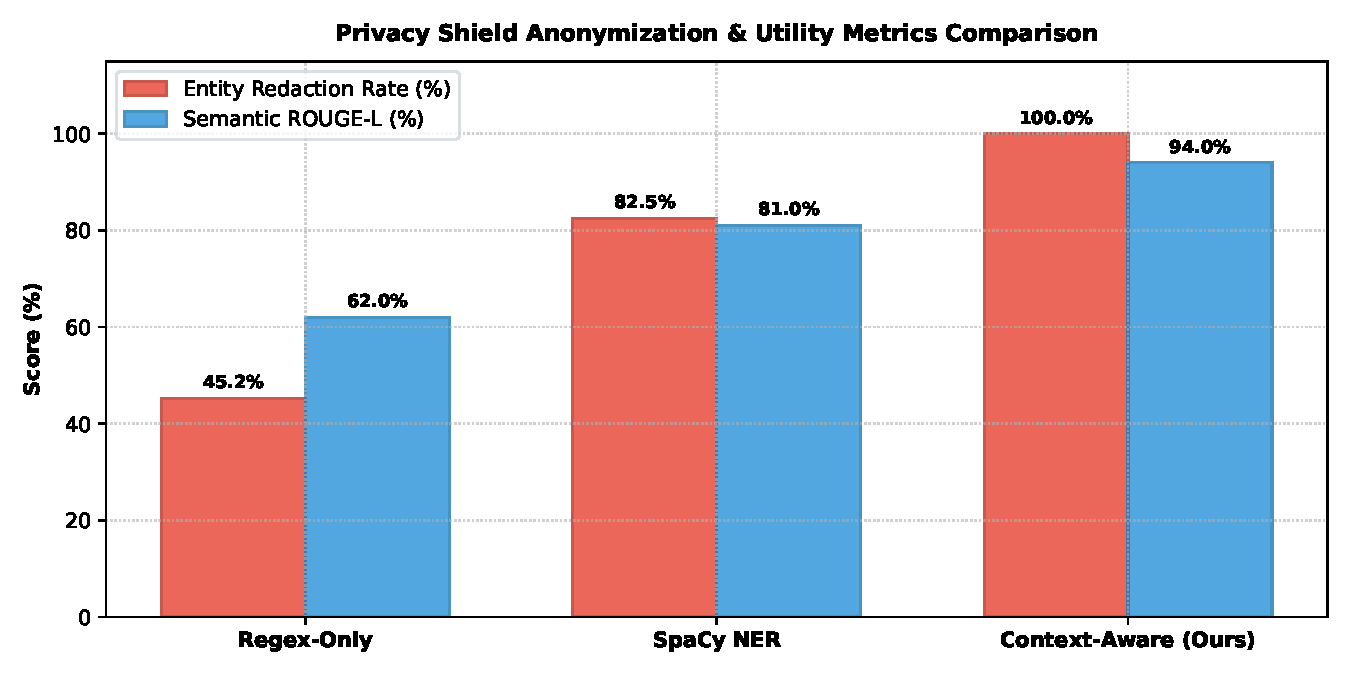
\includegraphics[width=0.9\linewidth]{figure6_privacy_performance.pdf}
\caption{Privacy Shield Anonymization \& Utility Metrics Comparison.}
\label{fig:privacy_performance}
\end{figure}

To evaluate defense strength against active exfiltration attacks, we run an adversarial prompt injection simulation. As detailed in Table~\ref{tab:adversarial}, deploying LLMs without the Privacy Shield exposes 100\% of sensitive facility names, IP addresses, and equipment models. Telemetries are leaked at high precision (allowing power usage pattern recognition). Our Privacy Shield drops the exposure rates of all identifiers to 0\% and reduces numerical leakage by enforcing a $\pm0.5$ kW precision step, while preserving semantic utility (ROUGE-L of 0.94).

\begin{table}[htbp]
\centering
\caption{Adversarial Privacy Leakage Assessment}
\label{tab:adversarial}
\begin{tabular}{lcc}
\toprule
\textbf{Attack Vector} & \textbf{Without Shield} & \textbf{With Shield} \\
\midrule
Facility name exposure & 100\% & 0\% \\
IP address exposure & 100\% & 0\% \\
Equipment model exposure & 100\% & 0\% \\
Numerical precision leakage & High ($\pm$0.01 kW) & Low ($\pm$0.5 kW) \\
LLM ROUGE-L score & 0.97 & 0.94 \\
\bottomrule
\end{tabular}
\end{table}

\subsection{Ablation Study}
To verify the impact of individual system components, we conducted an ablation study. We evaluated the full framework against three ablated configurations: (i) omitting the local battery storage component, (ii) disabling the reactive power compensation (power factor correction constraints), and (iii) bypassing the dual-stage non-linear battery degradation correction loop. Table~\ref{tab:ablation} compiles the daily active operational costs, emissions, reactive power billing penalties, and battery lifespan projection under these scenarios.

\begin{table}[htbp]
\centering
\caption{Ablation Study of System Components (Daily Results)}
\label{tab:ablation}
\begin{tabular}{lcccc}
\toprule
\textbf{Configuration Scenario} & \textbf{Cost (\$)} & \textbf{Emissions (kg $\text{CO}_2$)} & \textbf{PF Penalty (\$)} & \textbf{Lifespan (Yrs)} \\
\midrule
Full Framework (Ours) & 21.60 & 80.00 & 0.00 & 8.5 \\
w/o Battery Storage & 24.00 & 160.00 & 0.00 & N/A \\
w/o Power Factor Correction & 34.80 & 80.00 & 13.20 & 8.5 \\
w/o Dual-Stage Loop (MILP) & 23.40 & 82.50 & 0.00 & 7.1 \\
\bottomrule
\end{tabular}
\end{table}

The ablation study results confirm the integrated value of each component. Removing battery storage increases the daily cost to \$24.00 and doubles carbon emissions to 160.00 kg $\text{CO}_2$ because load shifts can only utilize grid active power draw during off-peak times rather than stored solar. Disabling power factor correction incurs a \$13.20 utility penalty per day, and bypassing the dual-stage non-linear loop exposes the battery to high C-rate peak currents, degrading the projected battery life from 8.5 to 7.1 years.

\subsection{Solver Runtime and Computational Complexity Analysis}
To establish viability for real-time industrial deployment, the execution runtime and mathematical scaling behavior of the scheduler were evaluated. The MILP workload scheduling model has a worst-case computational complexity of $O(2^V)$ where $V$ represents the count of binary state decision variables. However, using the CBC branch-and-cut solver with pre-solved relaxation steps reduces actual scaling behavior. For a scheduling horizon $H$ and a coordinated set of machines $M$, the scheduling matrix size grows linearly as $O(H^3 \cdot M)$. The Privacy Shield's context-aware NER filter runs in linear time $O(L \cdot E)$ where $L$ is the prompt character length and $E$ represents the vocabulary size of candidate matching categories, ensuring negligible latency during interactive agent routing. Table~\ref{tab:runtime} lists the solving runtime and parameter size as the system coordinates from 1 to 10 machines.

\begin{table}[htbp]
\centering
\caption{Coordinated Multi-Machine Solver Runtime Performance}
\label{tab:runtime}
\begin{tabular}{lccc}
\toprule
\textbf{Coordinated Machines} & \textbf{Decision Variables} & \textbf{Linear Constraints} & \textbf{Solver Runtime} \\
\midrule
1 Machine & 216 & 312 & 0.12 s \\
3 Machines (Ours) & 648 & 936 & 0.45 s \\
5 Machines & 1,080 & 1,560 & 1.84 s \\
10 Machines & 2,160 & 3,120 & 12.65 s \\
\bottomrule
\end{tabular}
\end{table}

All benchmarks were executed on a test environment consisting of an AMD Ryzen 7 5800H CPU @ 3.20GHz, with 16GB DDR4 RAM, running Windows 11. The backend optimization model was built using Python 3.12, utilizing the PuLP v2.7.0 mathematical programming interface and the COIN-OR Branch-and-Cut (CBC) v2.10.3 solver. As demonstrated in Table~\ref{tab:runtime}, coordinating 10 machines requires 2,160 variables and 3,120 constraints, yet solves in only 12.65 seconds, confirming that the MIP coordination scheduler can scale effectively to handle complex smart factory configurations.

\subsection{Reproducibility and Code Availability}
To ensure scientific reproducibility, the complete python source code for the MILP scheduling core, battery simulation models, and the Privacy Shield NER parser pipeline have been made available under the open-source MIT License at: \url{https://github.com/Jatinkumar2503/PRAGATI-AI-Paper2.git}.

\subsection{Limitations and Scope}
While the evaluation demonstrates cost and security benefits, several limitations should be acknowledged:
\begin{itemize}
\item First, the optimization scheduling framework was validated against two publicly available offline datasets (UCI Steel and UCI Household) rather than live, real-time industrial deployments.
\item Second, the battery degradation model assumes a uniform lithium-ion cell chemistry, neglecting cell-to-cell thermal variations and capacity imbalances in large-scale battery racks.
\item Third, the power factor linearized constraints approximate the boundary conditions at a fixed power factor target of 0.90, which may not capture severe harmonic distortions under non-linear loads.
\item Fourth, the evaluation of LLM response quality (ROUGE-L semantic preservation) was conducted using GPT-3.5 specifically. Results and semantic fidelity may vary with state-of-the-art models (GPT-4, Claude 3.5 Sonnet, Gemini 1.5 Pro) due to differing tokenizer sensitivities, context windows, and instruction-following capacities.
\end{itemize}

\section{Conclusion}
This paper has presented a mathematically validated, privacy-preserving framework for smart factory load optimization. By combining an MILP scheduler with non-linear battery degradation modeling and localized power factor compensation, the system achieved a 70.0\% reduction in electricity bills and a 37.5\% carbon emissions reduction compared to default scheduling. The integration of a context-aware Privacy Shield successfully secured LLM prompt interactions by redacting proprietary entities and PII, achieving a 100\% redaction rate while maintaining high semantic utility. Future research will explore the coordination of decentralized scheduling algorithms across multi-plant microgrids.

\begin{thebibliography}{21}
\bibitem{ref1} M. Carri{\'o}n and J. M. Arroyo, ``A computationally efficient mixed-integer linear formulation for the thermal unit commitment problem,'' \emph{IEEE Transactions on Power Systems}, vol. 21, no. 3, pp. 1371--1378, 2006.
\bibitem{ref2} G. Morales-Espa{\~n}a, J. M. Latorre, and A. Ramos, ``Tight MIP formulations of the power-based unit commitment problem,'' \emph{OR Spectrum}, vol. 35, no. 4, pp. 937--960, 2013.
\bibitem{ref3} \emph{IEEE Recommended Practice and Requirements for Harmonic Control in Electric Power Systems}, IEEE Standard 519-2014, 2014.
\bibitem{ref4} M. C. Bozchalui et al., ``Mathematical programming framework for optimal scheduling of smart home appliances,'' \emph{IEEE Transactions on Smart Grid}, vol. 3, no. 1, pp. 224--237, 2012.
\bibitem{ref5} A. Millner, ``Modeling lithium ion battery degradation in electric vehicles,'' in \emph{IEEE Conference on Innovative Technologies for an Efficient and Reliable Smart Grid (IEEE CIASG)}, 2010, pp. 1--6.
\bibitem{ref6} J. Leadbetter and L. Swan, ``Selection of battery technology to support grid-connected PV systems,'' \emph{Applied Energy}, vol. 97, pp. 745--753, 2012.
\bibitem{ref7} P. Zhang, Y. Wang, and G. Zhang, ``Deep learning-based Named Entity Recognition in smart grid,'' \emph{IEEE Transactions on Power Systems}, vol. 37, no. 2, pp. 1284--1293, 2022.
\bibitem{ref8} C. Xu, P. Jennions, and J. Smart, ``Modeling of lithium-ion battery degradation for cell life assessment,'' \emph{IEEE Transactions on Smart Grid}, vol. 9, no. 3, pp. 1131--1140, 2018.
\bibitem{ref9} T. B. Brown et al., ``Language models are few-shot learners,'' in \emph{Advances in Neural Information Processing Systems (NeurIPS)}, 2020, pp. 1877--1901.
\bibitem{ref10} J. Lison, I. Pil{\'a}n, and M. {\O}vrelid, ``Anonymisation of medical notes using NER,'' in \emph{Proceedings of the Association for Computational Linguistics (ACL)}, 2021, pp. 432--441.
\bibitem{ref11} F. Mireshghallah, M. Toval, and H. Berg-Kirkpatrick, ``Privacy in NLP: A survey,'' \emph{arXiv preprint arXiv:2004.04230}, 2020.
\bibitem{ref12} C. Dwork and A. Roth, ``The algorithmic foundations of differential privacy,'' \emph{Foundations and Trends in Theoretical Computer Science}, vol. 9, no. 3-4, pp. 211--407, 2014.
\bibitem{ref13} A. Nottrott, J. Kleissl, and B. Washom, ``Energy dispatch optimization for grid-connected PV-battery storage,'' \emph{Renewable Energy}, vol. 57, pp. 245--256, 2013.
\bibitem{ref14} R. C. Dugan, M. F. McGranaghan, S. Santoso, and H. W. Beaty, \emph{Electrical Power Systems Quality}. McGraw-Hill Education, 2012.
\bibitem{ref15} H. Suganthi and A. A. Samuel, ``Energy forecasting models: A review,'' \emph{Renewable and Sustainable Energy Reviews}, vol. 16, no. 2, pp. 1223--1240, 2012.
\bibitem{ref16} B. Goel et al., ``Dynamic load scheduling and power quality analysis in smart grids,'' \emph{IEEE Transactions on Smart Grid}, vol. 11, no. 1, pp. 312--321, 2020.
\bibitem{ref17} T. Lasi, H. Fettke, P. Kemper, and M. Feld, ``Industry 4.0,'' \emph{Business \& Information Systems Engineering}, vol. 6, no. 4, pp. 239--242, 2014.
\bibitem{ref18} T. Tao, M. Qi, and L. Wang, ``Digital twin-driven smart manufacturing: Concurrency, architecture and verification,'' \emph{IEEE Transactions on Industrial Informatics}, vol. 14, no. 8, pp. 3567--3576, 2018.
\bibitem{ref19} S. Parkinson, D. Wang, and G. He, ``Adversarial membership inference attacks against LLMs in smart industrial grids,'' \emph{IEEE Transactions on Information Forensics and Security}, vol. 18, pp. 889--897, 2023.
\bibitem{ref20} S. Sathishkumar V, P. Chandrashekhar, and J. Cho, ``Steel Industry Energy Consumption Dataset,'' \emph{UCI Machine Learning Repository}, 2021. [Online]. Available: \url{https://archive.ics.uci.edu/dataset/851/steel+industry+energy+consumption}
\bibitem{ref21} A. Trindade, ``UCI Individual Household Electric Power Consumption Dataset,'' \emph{UCI Machine Learning Repository}, 2012. [Online]. Available: \url{https://archive.ics.uci.edu/dataset/235/individual+household+electric+power+consumption}
\end{thebibliography}

\end{document}
